\section{Overview}
In this chapter we will present in detail the planning and approach we followed to establish the studies and analyze their results. Two studies, a controlled one, followed by a non-controlled one were conducted with the participation of 9 undergraduate master's degree and third-year bachelor's degree students enrolled in the "Embedded Systems" course at the University of Salerno in Italy. Participation in the studies was agreed upon by the students and was voluntary.

Before taking part in the first study, a set of lectures and training sessions was held with the objective of training the participants on the topics tackled by the studies, namely unit testing, test scaffolding and TDD.



\section{Research Questions}
The study we performed aimed at answering the following Research Questions (\rqs)
As for the baseline experiment, and following the main research question introduced in the introduction section of this thesis, we defined the main goal of this study by applying the Goal Question Metrics template [1].



The main goal for the baseline experiment is therefore defined as follows:
\noindent
\textbf{Analyze} the use of \tdd 
\textbf{for the purpose of} evaluating its effects in the development of \ess
\textbf{with respect to} the quality of produced source code and its complexity and the developers' productivity 
\textbf{from the point of} view of the researcher and lecturer 
\textbf{in the context of} an \es course involving second year Master students in Computer Science.

According to this objective, three research questions were defined:
\begin{itemize}
    \item \textbf{RQ1.} Does the use of \tdd affect the quality of the solution to a programming task? 
    \textit{Aim}: We defined this \rq to understand if (and possibly to what extent) the use of \tdd with respect to \yw makes a difference with respect to quality of the written source code. An answer to RQ1 would have practical implications within the Agile community. For example, in case the use of \tdd positively affects source code quality, lecturers can teach \tdd in \es courses so spreading Agile in the academic context and then facilitating the adoption of this approach in the industrial context. In other words, if the newcomers of the working market are familiar with \tdd, and it is shown that it produces better quality source code for \ess, the software industry could be encouraged to migrate their development from \yw to \tdd.
    \item \textbf{RQ2.} Does the use of \tdd affect the complexity of the solution to a programming task?
    \textit{Aim}: With this RQ, we intend to understand if (and possibly to what extent) the complexity of the source code—how difficult to understand it is from the developer's perspective—of an \es is affected by the development approach (\tdd vs. \yw). The answer to this question helps us to better understand \tdd applied to the development of \ess from a different perspective. For example, the researcher could be interested to study the extent with which the quality of the source code of an \es affects software maintenance and evolution. A positive answer to RQ2 could justify this research direction.
    \item \textbf{RQ3.} Does the use of \tdd increase developers' productivity?
    Aim: We defined this RQ to understand if (and possibly to what extent) there is an effect of \tdd on the developers’ productivity. The answer to RQ3 helps us to better understand \tdd in the development of \ess companies operating in the context of the development of \ess could be encouraged to use TDD in case: (\textit{i}) there is an evidence that this approach improves productivity and (\textit{ii}) developers are familiar with this approach before being hired (e.g., \tdd has been learned at university).
\end{itemize}



\section{Experimental Units}
The participants for these studies were students at the University of Salerno, in Italy; they were a mix of second-year master's degree students in Salerno, and students visiting the university by means of the Erasmus program; this last group was further made up of master's degree students and third-year bachelor's degree students. Both groups were enrolled in the \textit{Embedded Systems} course at the University of Salerno. As for the master's students, not all of them had a computer science background (bachelor's degree).

The \textit{Embedded Systems} course covered the following topics: \dots but no TDD, which was in turn covered by the lectures and training sessions preceding the studies.

Participating in the studies was voluntary; the students were informed that any gathered data would be treated anonymously and shared for research purposes only; furthermore, participation would not directly affect their final mark for the Embedded System course; however, in order to encourage student participation, those who took part in the studies were rewarded with a bonus in their final mark. Among the students taking the course, 9 participated.

The participants for the tasks were asked to carry out their assignment by either using TDD or NO-TDD (i.e., any approach they preferred, except for TDD) depending on the group they were partitioned in. and on the period the task took place.



\section{Experimental Objects}
The experimental objects for the studies were three code katas, programming exercises aimed at practicing a technique or a programming language. As for the baseline studies, the two experimental objects implemented by the participants are the following:
\begin{itemize}
    \item \textbf{IntelligentOffice}: the goal is to develop a system which allows the user to manage the light, window blinds, and air quality level inside an office.
    \item \textbf{CleaningRobot}: the goal is to develop a system to control a cleaning robot which moves in a room and cleans the dust on the floor along the way. 
\end{itemize}

As for the replication experiment, the implemented task is:
\begin{itemize}
    \item \textbf{SmartHome}: the goal is to develop an intelligent system to manage various aspects of room inside a house.
\end{itemize}

Further details on the experimental objects, including user stories, hardware used, and other information, are provided as an appendix to this thesis.


\subsection{IntelligentOffice}

\subsection{CleaningRobot}

\subsection{SmartHome}




\section{Variables}
The participants were asked to carry out each task by using either \tdd or the approach they preferred (i.e., NO-TDD), therefore one of the independent variables considered is \textbf{Condition}, a nominal variable assuming two values, \tdd and \notdd. The data was collected over two periods for the controlled study, and over an additional period for the non-controlled study, so a second independent variable is \textbf{Period}, assuming the values $P1, P2, and P3$. During the three periods both treatments (\tdd or \notdd) were applied. Finally, since the participants were split into two groups, the last independemt variable is \textbf{Group}, which can assume the values G1 and G2.


As for the dependent variables considered in the studies, these are: \textbf{QLTY}, \textbf{PROD}, \textbf{TEST}, \textbf{CYC}, \textbf{COG}, \textbf{LOC}.
The variables QLTY, PROD and TEST have been used in previous empirical studies \cite{DBLP:journals/tse/ErdogmusMT05}, \cite{DBLP:journals/tse/FucciETOJ17}, \cite{DBLP:journals/ese/TosunDFVTESOTJJ17}. As for the others, \dots

QLTY quantifies the external quality of the solution a participant implemented. It is formally defined as follows: 
\[
    QLTY = \frac{\sum_{i=1}^{\#TUS} QLTY_i}{\#TUS} * 100 
\]
where $\#TUS$ is the number of user stories a participant tackled, while $QLTY_i$ is the external quality of the $i-th$ user story; to determine whether a user story was tackled or not, the asserts in the test suite corresponding to the story were checked: if at least one assert in the test suite for the story passed, than the story was considered as tackled. $\#TUS$ is formally defined as follows:
\[
    \#TUS = \sum_{i=1}^{n} 
        \begin{cases}
            1 & \text{$\#ASSERT_i(PASS) > 0$}\\
                0 & \text{otherwise}
        \end{cases}
\]
Finally, the quality of the $i-th$ user story (i.e., $QLTY_i$) is defined as the ratio of asserts passed for the acceptance suite of the $i-th$ user story over the total number of asserts in the acceptance suite for the same story. More formally:
\[
    QLTY_i = \frac{\#ASSERT_i(PASS)}{\#ASSERT_i(ALL)}
\]
As a result, the $QLTY$ measure deliberately excludes unattempted tasks and tasks with zero success; therefore, it represents a local measure of external quality calculated over the subset of user stories that the subject attempted. $QLTY$ is a ratio measure in the range $[0, 100]$.

PROD estimates the productivity of a participant. It is computed as follows:
\[
    PROD = \frac{\#ASSERT(PASS)}{\#ASSERT(ALL)} * 100
\]
where $ASSERT(PASS)$ is the total number of asserts that have passed, by considering all acceptance test suites, while $ASSERT(ALL)$ refers to the total number of asserts in the acceptance suites. The $PROD$ variable can assume values between 0 and 100, where a value close to 0 indicates low productivity in the implemented solution, while a value close to 1 refers to high productivity.

The TEST variable quantifies the number of unit tests a participant wrote. It is defined as the number of assert statements in the test suite written by the participant; this variable ranges from 0 to $\infty$.


As for the additional three dependent variables regarding the general code quality in the submitted projects, these are defined as follows:
(\textbf{$CYC$}) refers to the Cyclomatic Complexity of the implemented solution; it is a value used to determine the stability and level of confidence in a program, and it measures the number of linearly-independent paths inside a program module. A program with a lower Cyclomatic Complexity is generally easier to understand and less "risky" to modify; it can be used as an estimate on how difficult the code will be to cover/test.

(\textbf{$COG$}) is the Cognitive Complexity of the solution; it is a measurement of how difficult a program module is to intuitively understand. A method's Cognitive Complexity is based on a few rules \cite{CognitiveComplexity}:
\begin{enumerate}
    \item Code is not considered more complex when it uses shorthand syntax that the language provides for collapsing multiple statements into one.
    \item Code is considered more complex for each "break in the linear flow of the code".
    \item Code is considered more complex when "flow breaking structures are nested"
\end{enumerate}

Finally, $LOC$ is the total number of lines of code written by the participant; it's defined as the sum of the individual lines of code in both the production code source file and the test code source file.



\section{Study design}
For the controlled baseline experiment, the participants were randomly split into two groups, G1 and G2, having 4 and 5 members respectively. For the first period P1, the group G1 was assigned the \tdd version of the first task, \textit{IntelligentOffice}, while the group G2 was assigned the \notdd version; on the other hand, during period P2, the group G1 was assigned the \notdd version of the second task, \textit{CleaningRobot}, while the group G2 was assigned the \tdd version.
Therefore, the design of our study can be classified as a repeated-measures, within-subjects design. In each period, the participants in G1 and G2 dealt with different experimental objects, therefore, at the end of the study, every participant had tackled each experimental object only once.

As for the replication study, the group structure remained the same, however each participant was randomly assigned the \tdd or \notdd version of the third and final experimental task, \textit{SmartHome}.


\section{Procedure}
Before our study took place, we collected some demographic information on the participants. To this end, the participants were asked to fill out an on-line pre-questionnaire (created by means of Google Forms).

The \textit{Embedded Systems} course, during which the study was conducted, started in September 2022. The first task, P1, took place on Tuesday, December 6th 2022, while the second, P2, took place on Tuesday, December 13th 2022.

Between the start of the course and P1, most participants had never dealt with \tdd, while they were somewhat familiar with unit testing and iterative test-last development. 
In the weeks prior to P1, \tdd was introduced to the participants via some frontal lectures and training/homework sessions.

The schedule for the training was as follows:
\dots

After each period of the controlled baseline study, participants were asked to fill out another on-line questionnaire, with the purpose of describing their general experience with the implementation of the task, focusing on their testing approach. 
The structure of the post-questionnaires was made up of three interval scale questions, and a variable number of open-ended questions, two for the \tdd group and three for the \notdd, with the latter having an additional question, as the first open-ended question, asking to provide information about the chosen approach for testing. Furthermore, the post-questionnaire presented at the end of period P2 contained an additional open question: here, participants had to provide their feelings towards both testing practices, \tdd and \notdd. 

More specifically, the interval scale questions were:
\begin{itemize}
    \item \textbf{Q1.} Regarding the comprehensibility of the provided user stories, I have found them: (Very unclear $|$ Unclear $|$ Neither clear nor unclear $|$ Clear $|$ Very clear).
    \item \textbf{Q2.} I have found the development task: (Very difficult $|$ Difficult $|$ Neither easy nor difficult $|$ Easy $|$ Very easy).
    \item \textbf{Q3.} Applying (\ie \tdd or \notdd) to accomplish the development task has been: (Very difficult $|$ Difficult $|$ Neither easy nor difficult $|$ Easy $|$ Very easy).
\end{itemize}

\noindent As for the open-ended questions:
\begin{itemize}
    \item (\textbf{\notdd only}) Describe the no-TDD approach you have followed to accomplish the development task.
    \item Provide your feelings (both positive and negative) about (\ie \tdd or \notdd).
    \item Provide your feelings (both positive and negative) about the development task.
    \item (\textbf{Task 2 only}) After applying (\ie \tdd or \notdd) in the last exercise, do you have any thoughts on the differences between the two approaches and your preference for using one over the other?
\end{itemize}

\noindent No formal questionnaire was provided for the replication study; however, after the hardware deployment step, each participant was individually interviewed about their overall experience with the studies:
\begin{enumerate}
    \item Provide your feelings (both positive and negative) about the final development project, (\eg development pipeline, used technologies).
    \item Provide your feelings (both positive and negative) about the development approach (\ie \tdd or \notdd) used to accomplish the final development project:
        \begin{itemize}
            \item \tdd: did you perform any refactoring? 
            \item \notdd: did you test the code at all? If so, which approach did you use?
        \end{itemize}
    \item Provide your feelings about the overall training experience (seminars, exercises, and homework on \tdd and \notdd, experiments, and final task):
        \begin{itemize}
            \item Positive and negative points and challenges encountered when applying TDD
            \item What can be done to improve the application of TDD in the development of \ess
            \item Please provide a discussion on \tdd vs. \notdd in the development of \ess
        \end{itemize}
\end{enumerate}
 




\section{Analysis Methods}
\begin{enumerate}
    \item \textbf{Individual analysis}
    \item \textbf{Aggregate analysis}:
\end{enumerate}
Meta-analysis is a research process used to systematically synthesize or merge the findings of single, independent studies, using statistical methods to calculate an overall or "absolute" effect. This kind of analysis does not simply pool data from smaller studies to achieve a larger sample size: analysts use well recognized, systematic methods to account for differences in sample size, variability (heterogeneity) in study approach and findings (treatment effects) and test how sensitive their results are to their own systematic review protocol (study selection and statistical analysis).




\section{Results}
\subsection{.}
In this section we will report the values observed for each dependent variable.
Besides the tables, box plot charts will be used to visualize the values assumed by the dependent variables.
A box plot chart is a type of chart often used in explanatory data analysis; it visually shows the distribution of numerical data and skewness through displaying the data quartiles (or percentiles) and averages.

Box plot definitions:
\begin{itemize}
    \item \textbf{Minimum value}: the lowest value, excluding outliers (shown at the end of the lower whisker).
    \item \textbf{Maximum value}: the highest score, excluding outliers (shown at the end of the upper whisker).
    \item \textbf{Median}: marks the mid-point of the data and is shown by the line that divides the box into two parts. Half the values are greater than or equal to this value and half are less than this value.
    \item \textbf{Inter-quartile range}: The middle “box” represents the middle 50\% of values for the group. The range of values from lower to upper quartile is referred to as the inter-quartile range. The middle 50\% of scores fall within the inter-quartile range.
    \item \textbf{Upper quartile}: 75\% of the scores fall below the upper quartile.
    \item \textbf{Lower quartile}: 25\% of scores fall below the lower quartile.
    \item \textbf{Whiskers}: the upper and lower "whiskers" represent scores outside the middle 50\% (i.e. the lower 25\% of scores and the upper 25\% of scores).
    \item \textbf{Outliers}: observations that are numerically distant from the rest of the data. They are defined as data points that are located outside the whiskers of the box plot, and are represented by a dot.
\end{itemize}

\noindent To provide an example of the kind of information that a box plot chart can provide, please consider the following figure displaying four student groups' opinions on a subject:

\dots

Some observations that can be made include:
\begin{itemize}
    \item The box plot is comparatively short (see box plot  (2)). This suggests that overall the student have a high level of agreement and therefore the values are very similar between each other.
    \item The box plot is comparatively tall (see box plots (1) and (3)). This, on the other hand, suggests students hold quite different opinions about this aspect or sub-aspect.
    \item Obvious differences between box plots (see box plots (1) and (2), (1) and (3), or (2) and (4)). Any obvious difference between box plots for comparative groups is worthy of further investigation.
    \item The 4 sections of the box plot are uneven in size (see box plot (1)). This reveals that many students share a similar view at certain parts of the scale, but in other parts of the scale students are more variable in their views. A long upper whisker in the means that students views are varied among the most positive quartile group, and very similar for the least positive quartile group. 
    \item Same median, different distribution (see box plots (1), (2), and (3)). The medians, which generally tend to be close to the average, are at the same level. However, the box plots in these examples show very different distributions of views. It's always important to consider the pattern of the whole distribution of responses in a box plot.
\end{itemize}


\textbf{Boxplot da inserire appena smetto di litigare con le immagini in Latex. Per il momento sono in una cartella separata}

\noindent\textbf{Task 1}: The following tables display the values for the variables measured for the first experimental task, IntelligentOffice, for the two groups, by applying each of the two conditions.
\\ \  \\
\noindent
\begin{tabular}{ |p{2cm}||p{1.6cm}|p{1.6cm}|p{1.6cm}|p{1.6cm}|p{1.6cm}|p{1.6cm}| }
    \hline
        \multicolumn{6}{|c|}{Task 1 - TDD} \\
    \hline
        Metric & Min & Max & Mean & Median & Std \\
    \hline
        QLTY & 73 & 96 & 81.12 & 77.77 & 10.73 \\
        PROD & 72 & 96 & 83 & 82 & 10 \\
        TEST & 8 & 10 & 9.5 & 10 & 1 \\
        CYC & 21 & 28 & 24.75 & 25 & 2.87 \\
        COG & 14 & 25 & 19 & 18.5 & 4.69 \\
        LOC & 154 & 195 & 167 & 159.5 & 18.95 \\
    \hline
\end{tabular}
\\ \  \\
\noindent
\begin{tabular}{ |p{2cm}||p{1.6cm}|p{1.6cm}|p{1.6cm}|p{1.6cm}|p{1.6cm}|}
    \hline
        \multicolumn{6}{|c|}{Task 1 - NO-TDD} \\
    \hline
        Metric & Min & Max & Mean & Median & Std\\
    \hline
        QLTY & 65.55 & 82 & 75.35 & 78.77 & 7.43 \\
        PROD & 56 & 84 & 76 & 80 & 11.66 \\
        TEST & 0 & 12 & 3.8 & 0 & 5.49 \\
        CYC & 12 & 18 & 15.6 & 16 & 2.19 \\
        COG & 9 & 17 & 14 & 15 & 3 \\
        LOC & 74 & 157 & 111.6 & 100 & 33.69 \\
    \hline
\end{tabular}
\\ \  \\

\noindent \textbf{Task 2}: The following tables display the values for the variables measured for the second experimental task, CleaningRobot, for the two groups, by applying each of the two conditions.
\\ \  \\
\noindent
\begin{tabular}{ |p{2cm}||p{1.6cm}|p{1.6cm}|p{1.6cm}|p{1.6cm}|p{1.6cm}|}
    \hline
        \multicolumn{6}{|c|}{Task 2 - TDD} \\
    \hline
        Metric & Min & Max & Mean & Median & Std\\
    \hline
        QLTY & 0 & 100 & 74.44 & 100 & 43.31 \\
        PROD & 8 & 100 & 38.6 & 21 & 37.35 \\
        TEST & 0 & 13 & 5.4 & 3 & 5.12 \\
        CYC & 9 & 19 & 12 & 10 & 4.06 \\
        COG & 2 & 40 & 12.8 & 4.0 & 15.91 \\
        LOC & 80 & 203 & 128 & 115 & 45.61 \\
    \hline
\end{tabular}

\noindent
\begin{tabular}{ |p{2cm}||p{1.6cm}|p{1.6cm}|p{1.6cm}|p{1.6cm}|p{1.6cm}|}
    \hline
        \multicolumn{6}{|c|}{Task 2 - NO-TDD} \\
    \hline
        Metric & Min & Max & Mean & Median & Std\\
    \hline
        QLTY & 74 & 94.43 & 83.07 & 81.94 & 10.17 \\
        PROD & 52 & 73 & 60.5 & 58.5 & 10.24 \\
        TEST & 5 & 12 & 9 & 9.5 & 2.94 \\
        CYC & 16 & 36 & 23.5 & 21 & 9 \\
        COG & 11 & 49 & 29 & 28 & 15.57 \\
        LOC & 178 & 260 & 207.5 & 196 & 37.11 \\
    \hline
\end{tabular}
\\ \  \\

\textbf{Tasks 1 \& 2}: the following tables display the values for the variables measured for the first two experimental tasks, i.e., the controlled study, for the two groups, by applying each of the two conditions.
\\ \  \\
\noindent
\begin{tabular}{ |p{2cm}||p{1.6cm}|p{1.6cm}|p{1.6cm}|p{1.6cm}|p{1.6cm}|}
    \hline
        \multicolumn{6}{|c|}{Task 1 \& 2 - TDD} \\
    \hline
        Metric & Min & Max & Mean & Median & Std\\
    \hline
        QLTY & 0 & 100 & 77.41 & 82 & 31.52 \\
        PROD & 8 & 100 & 58.33 & 72 & 35.76 \\
        TEST & 0 & 13 & 7.22 & 8 & 4.26 \\
        CYC & 9 & 28 & 17.66 & 19 & 7.51 \\
        COG & 2 & 40 & 15.55 & 14 & 12.06 \\
        LOC & 80 & 203 & 145.33 & 154 & 39.97 \\
    \hline
\end{tabular}
\\ \  \\
\noindent
\begin{tabular}{ |p{2cm}||p{1.6cm}|p{1.6cm}|p{1.6cm}|p{1.6cm}|p{1.6cm}|}
    \hline
        \multicolumn{6}{|c|}{Task 1 \& 2 - NO-TDD} \\
    \hline
        Metric & Min & Max & Mean & Median & Std\\
    \hline
        QLTY & 65.55 & 94.43 & 78.78 & 78.77 & 9.11 \\
        PROD & 52 & 84 & 69.11 & 73 & 13.22 \\
        TEST & 0 & 12 & 6.11 & 7.0 & 5.08 \\
        CYC & 12 & 36 & 19.11 & 16 & 7.07 \\
        COG & 9 & 49 & 20.66 & 15 & 12.56 \\
        LOC & 74 & 260 & 154.22 & 157 & 60.32 \\
    \hline
\end{tabular}
\\ \  \\


\textbf{Tasks 3}: finally, these last tables display the values for the variables measured for the third experimental task (non-controlled study), SmartHome, for the two groups, by applying each of the two conditions.
\\ \  \\
\noindent
\begin{tabular}{ |p{2cm}||p{1.6cm}|p{1.6cm}|p{1.6cm}|p{1.6cm}|p{1.6cm}|}
    \hline
        \multicolumn{6}{|c|}{Task 3 - TDD} \\
    \hline
        Metric & Min & Max & Mean & Median & Std\\
    \hline
        QLTY & 85 & 100 & 95 & 100 & 7.07 \\
        PROD & 83.33 & 100 & 93.33 & 100 & 9.13 \\
        TEST & 7 & 18 & 11.6 & 12 & 4.15 \\
        CYC & 15 & 30 & 22.6 & 20 & 6.58 \\
        COG & 18 & 34 & 25.8 & 25 & 7.08 \\
        LOC & 150 & 232 & 187 & 175 & 36.15 \\
    \hline
\end{tabular}
\\ \  \\
\noindent
\begin{tabular}{ |p{2cm}||p{1.6cm}|p{1.6cm}|p{1.6cm}|p{1.6cm}|p{1.6cm}|}
    \hline
        \multicolumn{6}{|c|}{Task 3 - NO-TDD} \\
    \hline
        Metric & Min & Max & Mean & Median & Std\\
    \hline
        QLTY & 80 & 100 & 86.25 & 82.5 & 9.46 \\
        PROD & 75 & 100 & 83.33 & 79.16 & 11.78 \\
        TEST & 0 & 11 & 4.5 & 3.5 & 5.44 \\
        CYC & 16 & 23 & 19.5 & 19.5 & 2.88 \\
        COG & 19 & 25 & 21 & 20 & 2.70 \\
        LOC & 93 & 164 & 125.5 & 122.5 & 36.82 \\
    \hline
\end{tabular}
\\ \  \\


\subsection{Post-questionnaire Analysis}
Fig \ref{bar_charts} summarizes the answers provided by the participants in the post-experiment questionnaires, comparing the responses by the employed condition (\tdd or \notdd).
Regarding user story comprehensibility, in the first experimental task, \textit{IntelligentOffice}, the majority of participants have a similar agreement on the matter, with percentages of agreement of 88\% (\tdd) and 80\% (\notdd). As for the second task, \textit{CleaningRobot}, there is a more substantial difference, with only 40\% of the \tdd group having a positive perception of the user stories' comprehensibility, compared to the 87\% of the \notdd group.

A similar trend can be noted for the second question, regarding the general task feasibility; here, in the first experimental task, the participants somewhat agree, with 50\% of the \tdd group and 40\% of the \notdd group feeling neutral about the difficulty of the task. In the second task, the answers are quite mixed, with 40\% of the participants in the \tdd finding the task at hand very difficult to understand, and the other 60\% equally split between finding the task hard, feeling neutral about it or considering it very easy.  On the other hand, all of the participants in the \notdd group agreed on feeling neutral about their ease in developing it.

Finally, question three was focused on the difficulty of the participants in applying their reference condition (\ie \tdd or \notdd): for task 1, the \tdd group did not have a strong opinion on applying this technique, with 76\% feeling neutral about it, and the other 24\% finding the application of \tdd easy but not too easy; The \notdd group had also the majority of opinions feeling neutral about their approach (60\%), however this time 20\% of the participants felt very good about applying \notdd; this is probably due to their seniority with the approach.


\begin{figure}[htbp]
    \begin{subfigure}{\textwidth}
        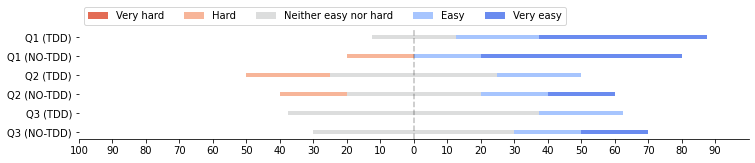
\includegraphics[width=\textwidth]{figures/bar_charts/task1.png}
        \caption{First experimental task, \textit{IntelligentOffice}}
    \end{subfigure}
    
    \bigskip
    
    \begin{subfigure}{\textwidth}
        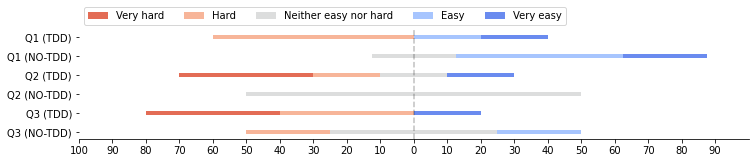
\includegraphics[width=\textwidth]{figures/bar_charts/task2.png}
        \caption{Second experimental task, \textit{CleaningRobot}}
    \end{subfigure}
    
    \caption{Diverging stacked bar charts for the post-questionnaires}
    \label{bar_charts}
\end{figure}


\section{Discussion}
\subsection{Answers to Research Questions}


\subsection{Implications}


\subsection{Threats to Validity}
In order to determine the potential threats to validity that may affect our studies, we referenced Wohlin \etal 's guidelines \cite{DBLP:books/sp/WohlinRHOR00}.




Completely avoiding/mitigating threats is often unfeasible, given the dependency between some threats: avoiding/mitigating a kind of threat (\ie  internal validity) might intensify or even introduce another kind of threat \cite{DBLP:books/sp/WohlinRHOR00}.

Generally, the kinds of threats to validity that can occur in a study can be classified in the following categories:
\begin{enumerate}
    \item \textbf{Threats to internal validity}. Internal validity the extent to which we can be confident that a cause-and-effect relationship established in a study cannot be explained by other factors; it makes the conclusions of a causal relationship credible and trustworthy. Without high internal validity, an experiment cannot demonstrate a causal link between two variables.
    There are three necessary conditions for internal validity and all three must occur to experimentally establish causality between an independent variable A (treatment variable) and dependent variable B (response variable):
    \begin{itemize}
        \item The treatment and response variables change together.
        \item The treatment precedes changes in the response variables
        \item No confounding or extraneous factors can explain the results of the study.
    \end{itemize}
    Threats to internal validity include: 
    \begin{itemize}
        \item \textbf{Selection bias}: groups are not comparable at the beginning of the study. For example, low-scorers were placed in Group A, while high-scorers were placed in Group B; Because there are already systematic differences between the groups at the baseline, any improvements in group scores may be due to reasons other than the treatment.
        \item \textbf{Regression to the mean}: there is a statistical tendency for people who score extremely low or high on a test to score closer to the middle the next time. Because participants are placed into groups based on their initial scores, it's hard to say whether the outcomes would be due to the treatment or statistical norms.
        \item \textbf{Social interaction and social desirability}: participants from different groups may compare notes and either figure out the aim of the study or feel resentful of others or pressured to act/react a certain way. For example, Groups B and C may resent Group A for some reason and, as such, they could be demoralized and perform poorly.
        \item \textbf{Attrition bias}: dropout from participants. For example, if 20\% of participants provided unusable data, and almost all of them were from Group C, it will be hard to compare the two treatment groups to a control group.
    \end{itemize}
    
    \item \textbf{Threats to external validity}: the extent to which we can generalize the findings of a study to other measures, settings or groups. In other words, can we apply the findings of your study to a broader context?
    Threats to external validity include: 
    \begin{itemize}
        \item \textbf{Sampling bias}: the sampling considered for the study is not representative of the average population. If the sample includes only people that participated in the study voluntarily, they could have characteristics that may make them very different from other populations, like people randomly chosen.
        \item \textbf{History}: an unrelated event influences the outcomes.
        \item \textbf{Observer bias}: the characteristics or behaviors of the experimenter(s) unintentionally influence the outcomes, leading to bias and other demand characteristics. For example, a trainer of the experimental sessions unintentionally reveals that the outcome of the study will influence their final mark. As a result, participants will work extra hard from that point on to ensure their result are the best possible.
        \item \textbf{Hawthorne effect}: the tendency for participants to change their behaviors simply because they know they are being studied. As an example, let's consider a set of participants that actively alters their behavior for the period of the study because they are conscious of their participation in the research.
        \item \textbf{Testing effect}: the administration of a pre- or post-test, or the repetition of similar tasks affects the outcomes.
        \item \textbf{Aptitude-treatment}: interactions between characteristics of the group and individual variables together influence the dependent variable.
        \item \textbf{Situation effect}: factors like the setting, time of day, location, researchers' characteristics, etc. limit generalizability of the findings
    \end{itemize}
    \item \textbf{Threats to construct validity}
    \item \textbf{Threats to conclusion validity}
\end{enumerate}

As mentioned above, there are inherent trade-offs between validities: with internal and external validities for example, the more we control extraneous factors in your study, the less we can generalize our findings to a broader context.


As for our controlled and replication studies, let's consider the different threats individually:

\noindent\textbf{Threats to internal validity}.
The main threat is perhaps related to the monitoring of the participants during the replication study; since they accomplished the implementation of the task at home, before deploying it on hardware under our supervision, we cannot be sure of the means by the participants to accomplish the task; we can however assume that, given the fact that the final score of the \textit{Embedded Systems} course was not influenced in any way by the outcome of the task, the participants would have no reason to \dots
Besides this, a \textit{selection} threat might have affected the overall results of the experiments, given that volunteers are generally more motivated and engaged compared to the average population \cite{DBLP:books/sp/WohlinRHOR00}. Finally, another potential threat is \textit{resentful demoralization}, which arises in participants when they receive a less desirable treatment; this causes them to not behave as they normally would. This last threat holds in all three experimental tasks, since it is related to the nature of the adopted experimental design.

\noindent\textbf{Threats to external validity}.
The main external validity threat could be the one of \textit{interaction of selection and treatment}: since both Bachelor's and Master's student were involved in the study, some of the latter with no prior testing experience or even without a strong Computer Science background, the results could potentially not be applicable to professional developers. 

\noindent\textbf{Threats to construct validity}.
Although we did not disclose the purpose of our study to the participants during the experimental tasks, they might have tried to guess it, and adapted their behavior accordingly, arising a threat of \textit{hypotheses guessing}. Besides this, the threat of \textbf{evaluation apprehension} should have been fairly mitigated, since the participants knew that they would be awarded the bonus score for the course regardless of their performance in the study.

\noindent\textbf{Threats to conclusion validity}
In order to mitigate any potential threat of \textit{random heterogeneity of participants}, before staring the experimental tasks, we trained the participants with a series of frontal lectures and exercise, in order to uniform their knowledge on the techniques and technologies that they would have later used and make the two groups as homogeneous as possible. A threat of \textit{reliability of treatment implementation} might have occurred in tasks 1 and 2. For example, some participants might have followed \tdd more strictly than others; however, this should equally affect both experimental groups.